% PRISM course project presentation (10 to 12 minutes). Build: latexmk -xelatex slides.tex
% Numbers come from docs/handoff/data/*.csv; the charts in figures/ are made by scripts/make_slide_figures.py.
\documentclass[aspectratio=169,11pt]{beamer}

\IfFileExists{beamerthememetropolis.sty}{%
  \usetheme{metropolis}
  \metroset{progressbar=frametitle,numbering=fraction,sectionpage=none}
}{%
  \usetheme{default}
  \setbeamertemplate{navigation symbols}{}
  \setbeamertemplate{footline}[frame number]
}

\usepackage{graphicx}
\usepackage{booktabs}
\usepackage{tabularx}
\usepackage{xcolor}
\usepackage{tikz}
\usetikzlibrary{arrows.meta,positioning,calc}
\usepackage[numbers]{natbib}
\usepackage{appendixnumberbeamer}

\definecolor{accent}{HTML}{2a78d6}
\definecolor{muted}{HTML}{8a8985}
\definecolor{light}{HTML}{c9c7c1}
\definecolor{ink}{HTML}{1c1b19}
\definecolor{ink2}{HTML}{5f5d58}
\definecolor{paper}{HTML}{f6f5f2}
\setbeamercolor{background canvas}{bg=white}
\setbeamercolor{normal text}{fg=ink}
\setbeamercolor{frametitle}{bg=white,fg=ink}
\setbeamercolor{progress bar}{fg=accent,bg=light!50}
\setbeamercolor{title separator}{fg=accent}
\setbeamercolor{alerted text}{fg=accent}
\setbeamercolor{footline}{fg=muted}
\setbeamerfont{frametitle}{size=\Large}
\setbeamertemplate{itemize item}{\color{accent}\textbullet}
\graphicspath{{figures/}{../docs/handoff/figures/}}

% Hindi examples: Devanagari if the font is installed, else a transliteration.
\IfFontExistsTF{Noto Sans Devanagari}{%
  \newfontfamily\devanagarifont[Script=Devanagari,Scale=0.95]{Noto Sans Devanagari}%
  \newcommand{\hindi}[2]{{\devanagarifont #1}}%
}{%
  \newcommand{\hindi}[2]{\textit{#2}}%
}
\newcommand{\lat}[1]{{\normalfont #1}} % Latin letters inside Devanagari text
\newcommand{\prompt}[1]{{\ttfamily\footnotesize #1}}
\newcommand{\aside}[1]{{\small\color{ink2} #1}}
\newcommand{\define}[2]{{\small\textbf{#1}\;\color{ink2}#2}}

% Card styles for the puzzle and trap rows (one tikzpicture per row, so cards line up).
\tikzset{card/.style={fill=paper, rounded corners=5pt, inner sep=8pt, anchor=north west},
  stat/.style={fill=paper, rounded corners=5pt, inner sep=9pt, anchor=north west}}
\newcommand{\cardtext}[1]{\parbox[t][4.2cm][t]{2.85cm}{\raggedright #1}}
\newcommand{\stattext}[1]{\parbox[t][4.2cm][t]{3.75cm}{\centering #1}}
% One timeline row: \plan{start week}{end week}{row}{colour}{label}
\newcommand{\plan}[5]{%
  \fill[#4, rounded corners=2pt] (#1+0.06, -#3+0.3) rectangle (#2-0.06, -#3-0.3);
  \node[anchor=east, color=ink, font=\footnotesize] at (-0.1, -#3) {#5};}

\title{What Sparse Autoencoders Miss Is Task-Specific}
\subtitle{Mapping the blind spot across tasks and languages}
\author{[Student name]}   % student: fill in
\institute{[Course name]} % student: fill in
\date{October 2026}

\begin{document}

%------------------------------------------------------------------------------
\maketitle

%------------------------------------------------------------------------------
\begin{frame}{How we look inside a language model}
  \centering
  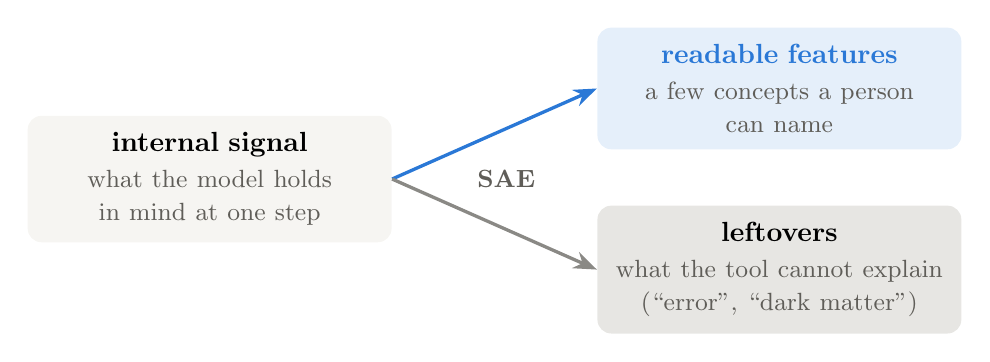
\begin{tikzpicture}[>=Stealth,
      box/.style={rounded corners=5pt, align=center, minimum height=1.5cm, text width=4.2cm, inner sep=6pt}]
    \node[box, fill=paper] (x) {\textbf{internal signal}\\[2pt]\aside{what the model holds\\in mind at one step}};
    \node[box, fill=accent!12, right=2.6cm of x, yshift=1.15cm] (f)
      {\textbf{\color{accent}readable features}\\[2pt]\aside{a few concepts a person\\can name}};
    \node[box, fill=light!45, right=2.6cm of x, yshift=-1.15cm] (e)
      {\textbf{leftovers}\\[2pt]\aside{what the tool cannot explain\\(``error'', ``dark matter'')}};
    \draw[->, very thick, accent] (x.east) -- (f.west);
    \draw[->, very thick, muted] (x.east) -- (e.west);
    \node[font=\small\bfseries, color=ink2] at ($(x.east) + (1.45,0)$) {SAE};
  \end{tikzpicture}

  \vspace{14pt}
  \define{Sparse autoencoder (SAE):}{the main tool researchers use to read a model's internal
    signal~\citep{bricken2023monosemanticity,cunningham2023sparse}.}
\end{frame}

%------------------------------------------------------------------------------
\begin{frame}{The idea in one slide}
  \centering
  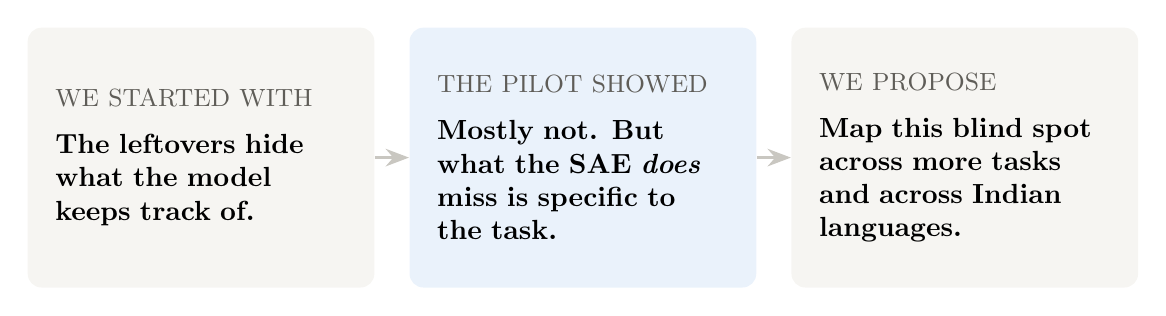
\begin{tikzpicture}[>=Stealth, idea/.style={fill=paper, rounded corners=5pt, text width=3.7cm, align=left,
      inner sep=10pt, minimum height=3.3cm, anchor=north}]
    \node[idea] (a) at (0,0) {{\small\color{ink2}WE STARTED WITH}\\[5pt]
      \textbf{The leftovers hide what the model keeps track of.}};
    \node[idea, fill=accent!10] (b) at (4.85,0) {{\small\color{ink2}THE PILOT SHOWED}\\[5pt]
      \textbf{Mostly not. But what the SAE \emph{does} miss is specific to the task.}};
    \node[idea] (c) at (9.7,0) {{\small\color{ink2}WE PROPOSE}\\[5pt]
      \textbf{Map this blind spot across more tasks and across Indian languages.}};
    \draw[->, very thick, light] (a.east) -- (b.west);
    \draw[->, very thick, light] (b.east) -- (c.west);
  \end{tikzpicture}
\end{frame}

%------------------------------------------------------------------------------
\begin{frame}{The swap test: does the right answer come back?}
  \centering
  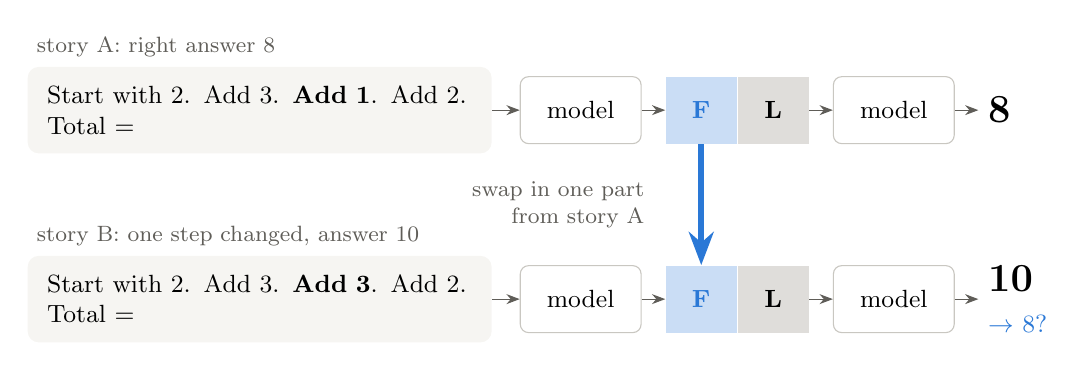
\begin{tikzpicture}[>=Stealth, font=\small,
      story/.style={fill=paper, rounded corners=4pt, align=left, text width=5.4cm, inner sep=7pt},
      blk/.style={draw=light, rounded corners=3pt, minimum height=0.85cm, align=center, text width=1.3cm},
      part/.style={minimum width=0.9cm, minimum height=0.85cm}]
    \node[story] (s1) at (0,0) {Start with 2. Add 3. \textbf{Add 1}. Add 2. Total =};
    \node[blk, right=0.35cm of s1] (m1) {model};
    \node[part, fill=accent!25, right=0.3cm of m1] (f1) {\color{accent}\bfseries F};
    \node[part, fill=light!60, right=0pt of f1] (e1) {\bfseries L};
    \node[blk, right=0.3cm of e1] (n1) {model};
    \node[right=0.3cm of n1, font=\Large\bfseries] (a1) {8};
    \node[story] (s2) at (0,-2.4) {Start with 2. Add 3. \textbf{Add 3}. Add 2. Total =};
    \node[blk, right=0.35cm of s2] (m2) {model};
    \node[part, fill=accent!25, right=0.3cm of m2] (f2) {\color{accent}\bfseries F};
    \node[part, fill=light!60, right=0pt of f2] (e2) {\bfseries L};
    \node[blk, right=0.3cm of e2] (n2) {model};
    \node[right=0.3cm of n2, font=\Large\bfseries, align=left] (a2) {10\\[-3pt]{\small\mdseries\color{accent}$\to$ 8?}};
    \foreach \a/\b in {s1/m1, m1/f1, e1/n1, n1/a1, s2/m2, m2/f2, e2/n2, n2/a2} \draw[->, ink2] (\a) -- (\b);
    \draw[->, line width=2pt, accent] (f1.south) -- (f2.north);
    \node[anchor=east, align=right, font=\footnotesize, color=ink2] at ($(f1.south)!0.5!(f2.north) + (-0.6,0)$)
      {swap in one part\\from story A};
    \node[font=\footnotesize, color=ink2, anchor=south west] at (s1.north west) {story A: right answer 8};
    \node[font=\footnotesize, color=ink2, anchor=south west] at (s2.north west) {story B: one step changed, answer 10};
  \end{tikzpicture}

  \vspace{10pt}
  \aside{\textbf{F} = readable features, \textbf{L} = leftovers. \;Score: \textbf{how much of the right answer comes back},
    from 0\% (still 10) to 100\% (back to 8). Swapping everything gives 100\%.}
\end{frame}

%------------------------------------------------------------------------------
\begin{frame}{Pilot: four puzzles the model can solve}
  \centering
  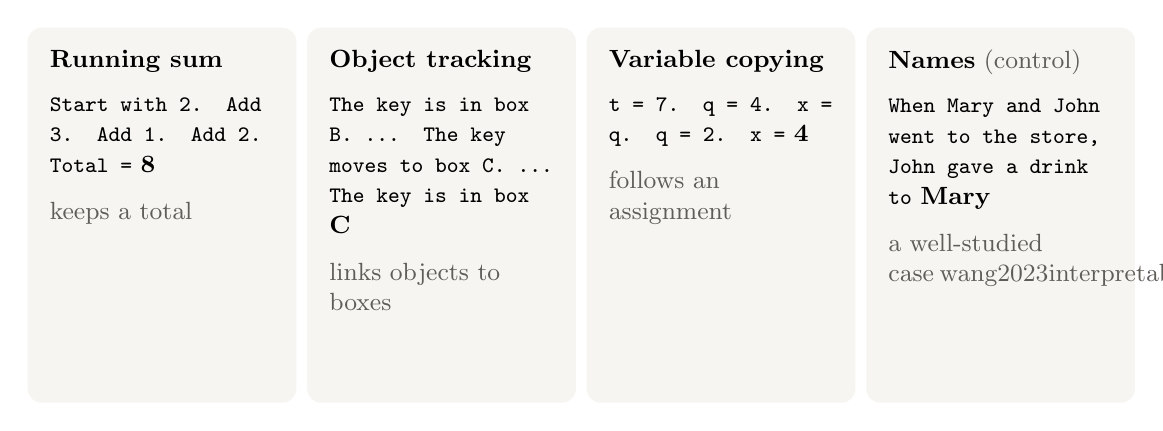
\begin{tikzpicture}[every node/.append style={font=\small}]
    \node[card] at (0,0) {\cardtext{\textbf{Running sum}\\[5pt]\prompt{Start with 2. Add 3. Add 1. Add 2. Total =}
      \textbf{8}\\[6pt]\aside{keeps a total}}};
    \node[card] at (3.55,0) {\cardtext{\textbf{Object tracking}\\[5pt]\prompt{The key is in box B. \dots{} The key moves to box C.
      \dots{} The key is in box} \textbf{C}\\[6pt]\aside{links objects to boxes}}};
    \node[card] at (7.1,0) {\cardtext{\textbf{Variable copying}\\[5pt]\prompt{t = 7. q = 4. x = q. q = 2. x =}
      \textbf{4}\\[6pt]\aside{follows an assignment}}};
    \node[card] at (10.65,0) {\cardtext{\textbf{Names} \aside{(control)}\\[5pt]\prompt{When Mary and John went to the store, John
      gave a drink to} \textbf{Mary}\\[6pt]\aside{a well-studied case~\citep{wang2023interpretability}}}};
  \end{tikzpicture}

  \vspace{10pt}
  \aside{Model: gemma-2-2b (Google) \;$\cdot$\; SAEs: Gemma Scope~\citep{lieberum2024gemmascope} \;$\cdot$\; 150 test
    pairs per puzzle \;$\cdot$\; three harder puzzles were dropped: the model could not solve them.}
\end{frame}

%------------------------------------------------------------------------------
\begin{frame}{Readable features carry most of the answer}
  \centering
  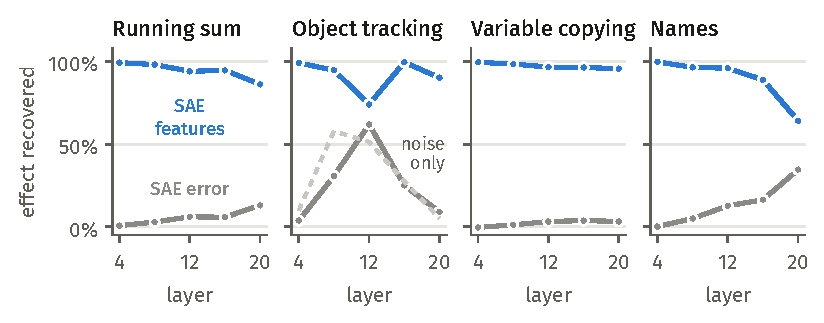
\includegraphics[width=\textwidth]{s_split.pdf}

  \vspace{6pt}
  \aside{The ``leftovers hide it'' idea is mostly wrong here. One exception stands out: object tracking, middle layers.}
\end{frame}

%------------------------------------------------------------------------------
\begin{frame}{Object tracking leaks: one hidden signal recovers half of it}
  \centering
  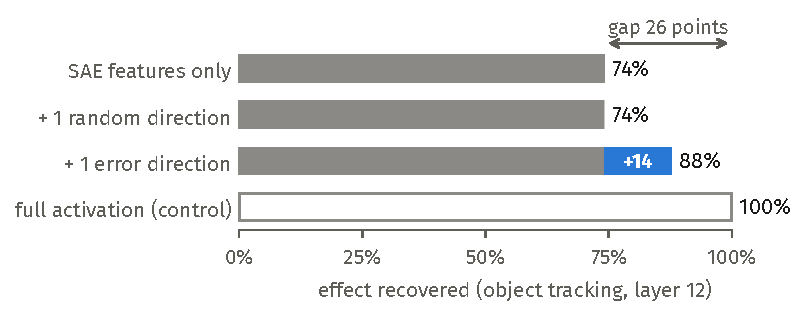
\includegraphics{s_gap.pdf}

  \vspace{6pt}
  \aside{The SAE misses 26\% of the answer. A single signal pulled from the leftovers brings 14 points back.}
\end{frame}

%------------------------------------------------------------------------------
\begin{frame}{The missing piece is specific to the task}
  \centering
  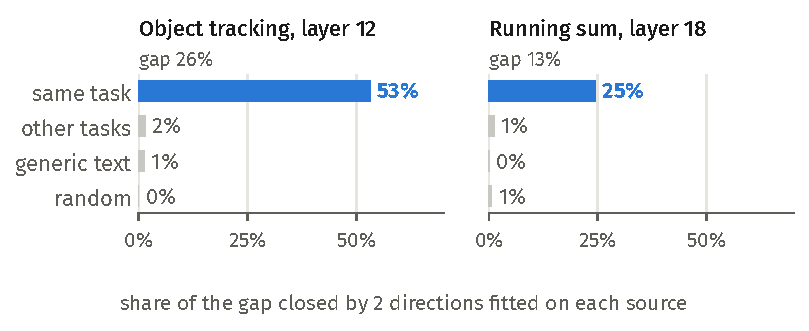
\includegraphics[width=\textwidth]{s_specific.pdf}

  \vspace{6pt}
  \aside{Signals learned from the same task fill the gap. Signals from other tasks or ordinary web text do almost nothing.}
\end{frame}

%------------------------------------------------------------------------------
\begin{frame}{A 16$\times$ bigger SAE shrinks the gap but does not close it}
  \centering
  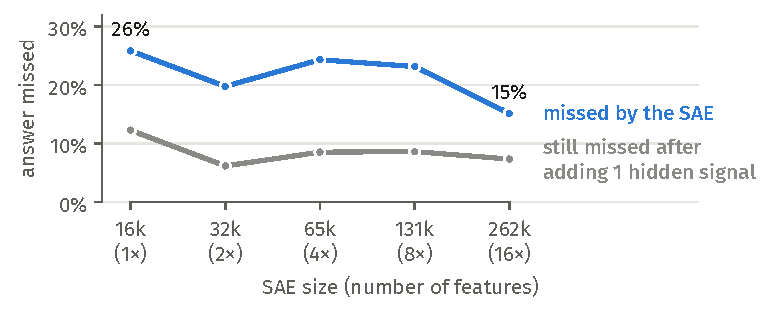
\includegraphics{s_width.pdf}

  \vspace{6pt}
  \aside{At every size, one hidden signal still recovers about half of what is missed.}
\end{frame}

%------------------------------------------------------------------------------
\begin{frame}{Three ways to fool yourself (we hit all three)}
  \centering
  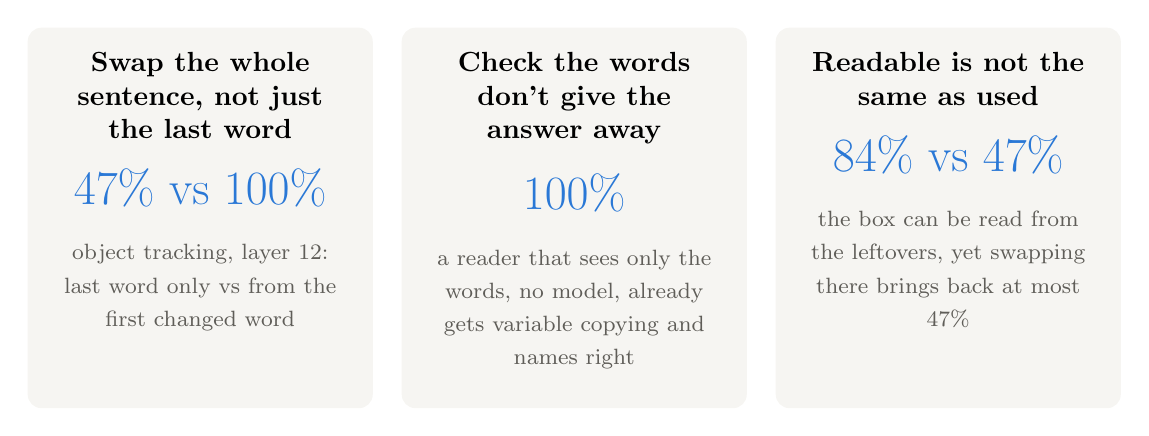
\begin{tikzpicture}
    \node[stat] at (0,0) {\stattext{\textbf{Swap the whole sentence, not just the last word}\\[10pt]{\LARGE\color{accent}47\% vs 100\%}\\[8pt]{\footnotesize\color{ink2}object tracking, layer 12: last word only vs from the first changed
      word}}};
    \node[stat] at (4.75,0) {\stattext{\textbf{Check the words don't give the answer away}\\[10pt]{\LARGE\color{accent}100\%}\\[8pt]
      {\footnotesize\color{ink2}a reader that sees only the words, no model, already gets variable copying and names
      right}}};
    \node[stat] at (9.5,0) {\stattext{\textbf{Readable is not the same as used}\\[10pt]{\LARGE\color{accent}84\% vs 47\%}\\[8pt]
      {\footnotesize\color{ink2}the box can be read from the leftovers, yet swapping there brings back at most
      47\%}}};
  \end{tikzpicture}
\end{frame}

%------------------------------------------------------------------------------
\begin{frame}{Next (1): map the effect across tasks}
  \small
  \renewcommand{\arraystretch}{1.35}
  \begin{tabularx}{\textwidth}{@{}l X l@{}}
    \toprule
    \textbf{Kind of task} & \textbf{Examples} & \textbf{Status} \\
    \midrule
    Linking things & objects in boxes; people and their cities\, \aside{(new)} & pilot + new \\
    Keeping a count & running sum; longer chains\, \aside{(new)} & pilot + new \\
    Following references & variable copying & pilot \\
    Control & names & pilot \\
    \bottomrule
  \end{tabularx}

  \vspace{10pt}
  For every task: \textbf{how much} does the SAE miss, \textbf{is it task-specific}, does a \textbf{bigger SAE} fix it?\\[4pt]
  \define{Binding test:}{is the leak the model's way of linking ``what goes with what''~\citep{feng2024bind}? Change only
    the hidden signal and see if the model names the other box.}
\end{frame}

%------------------------------------------------------------------------------
\begin{frame}{Next (2): does the SAE miss more in Indian languages?}
  \begin{columns}[T]
    \begin{column}{0.44\textwidth}
      \centering
      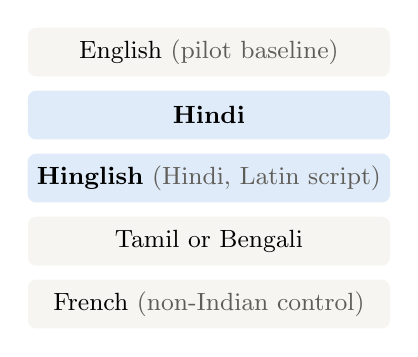
\begin{tikzpicture}[lang/.style={fill=paper, rounded corners=3pt, minimum width=4.6cm, minimum height=0.62cm,
          font=\small}]
        \node[lang] at (0,0) {English \aside{(pilot baseline)}};
        \node[lang, fill=accent!15] at (0,-0.8) {\textbf{Hindi}};
        \node[lang, fill=accent!15] at (0,-1.6) {\textbf{Hinglish} \aside{(Hindi, Latin script)}};
        \node[lang] at (0,-2.4) {Tamil or Bengali};
        \node[lang] at (0,-3.2) {French \aside{(non-Indian control)}};
      \end{tikzpicture}

      \vspace{8pt}
      \raggedright\aside{The SAEs were trained on mostly English text~\citep{lieberum2024gemmascope}.}
    \end{column}
    \begin{column}{0.54\textwidth}
      \small
      \textbf{Three questions}
      \begin{enumerate}\setlength{\itemsep}{2pt}
        \item Does the SAE explain Hindi text as well as English?
        \item Is the leak bigger in Hindi?
        \item Is it the same hidden signal? \aside{(learn it in English, test it in Hindi)}
      \end{enumerate}
      \vspace{6pt}
      \textbf{Same puzzles, translated} \aside{(illustrative, to be checked)}\\[3pt]
      \hindi{शुरुआत 2 से करें। 3 जोड़ें। 1 जोड़ें। 2 जोड़ें। कुल =}{shuruaat 2 se karen. 3 joden. 1 joden. 2 joden. kul =}
      \textbf{8}\\[2pt]
      \prompt{Jab Rahul aur Priya market gaye, Priya ne ek book di. Book kisko mili? Answer:} \textbf{Rahul}
    \end{column}
  \end{columns}
\end{frame}

%------------------------------------------------------------------------------
\begin{frame}{Plan: six weeks}
  \centering
  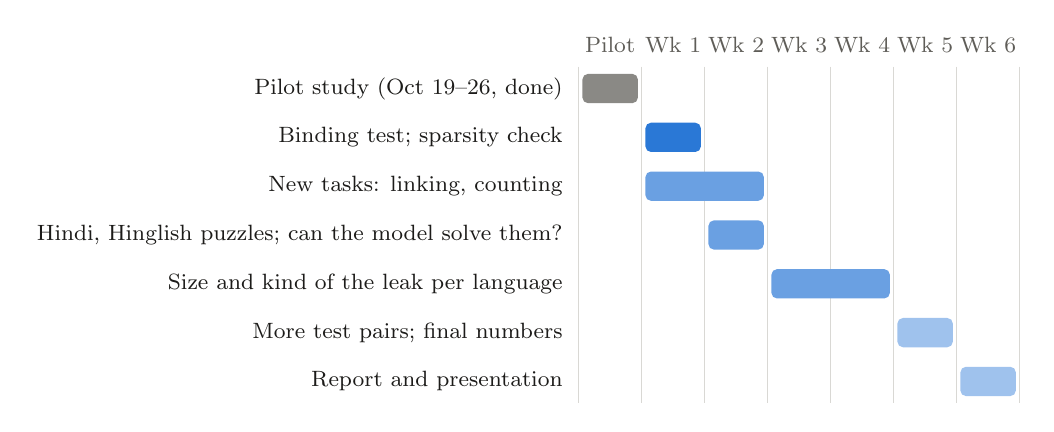
\begin{tikzpicture}[x=0.8cm, y=0.62cm, font=\small]
    \foreach \w/\l in {0/Pilot, 1/Wk 1, 2/Wk 2, 3/Wk 3, 4/Wk 4, 5/Wk 5, 6/Wk 6}
      \node[color=ink2, font=\footnotesize] at (\w+0.5, 0.9) {\l};
    \foreach \w in {0,...,7} \draw[light!70] (\w, 0.45) -- (\w, -6.45);
    \plan{0}{1}{0}{muted}{Pilot study (Oct 19--26, done)}
    \plan{1}{2}{1}{accent}{Binding test; sparsity check}
    \plan{1}{3}{2}{accent!70}{New tasks: linking, counting}
    \plan{2}{3}{3}{accent!70}{Hindi, Hinglish puzzles; can the model solve them?}
    \plan{3}{5}{4}{accent!70}{Size and kind of the leak per language}
    \plan{5}{6}{5}{accent!45}{More test pairs; final numbers}
    \plan{6}{7}{6}{accent!45}{Report and presentation}
  \end{tikzpicture}
\end{frame}

%------------------------------------------------------------------------------
\begin{frame}{Takeaways}
  \begin{enumerate}\setlength{\itemsep}{12pt}
    \item \textbf{SAEs keep most of what a model tracks.} Readable features bring back 74\% to 100\% of the answer.
    \item \textbf{What they miss is task-specific.} For object tracking, one hidden signal holds half the gap; signals
      from other tasks or ordinary text do not help, and a 16$\times$ bigger SAE does not remove it.
    \item \textbf{Next: map this blind spot} across more tasks and in Hindi and Hinglish.
  \end{enumerate}
\end{frame}

%==============================================================================
\appendix

\begin{frame}{Backup: the original claims and what the pilot found}
  \small
  \renewcommand{\arraystretch}{1.3}
  \begin{tabularx}{\textwidth}{@{}X X@{}}
    \toprule
    \textbf{Original claim} & \textbf{Pilot verdict} \\
    \midrule
    The leftovers carry what the model tracks & \textbf{Mostly no:} readable features bring back 74\% to 100\%;
      leftovers 0\% to 13\% (object tracking up to 62\%) \\
    The tracked state sits in the leftovers in a simple, readable shape & \textbf{Readable, not used:} a reader decodes it
      there (84\%), but the model does not use it at that spot yet \\
    A few hidden signals in the leftovers fill the gap & \textbf{Yes, narrowly:} one signal recovers about half of
      object tracking's 26\% gap; only for that task \\
    \bottomrule
  \end{tabularx}
\end{frame}

\begin{frame}{Backup: caveats}
  \small
  \begin{itemize}\setlength{\itemsep}{4pt}
    \item One model (gemma-2-2b), one SAE family (Gemma Scope), made-up puzzles.
    \item The names control also loses 24\% to 36\% in late layers, but that loss is spread over about 32 signals, so
      part of the late-layer loss is a general SAE weakness.
    \item Object tracking's ``leftovers only'' score (62\% at layer 12) is inflated: replacing the leftovers with noise
      already gives 51\%.
    \item The 131k and 262k SAEs also use more features per word (124 to 139 vs 75 to 89 at 16k), so part of the
      shrinking gap may come from that, not from size.
    \item The binding explanation and everything multilingual are plans, not results.
  \end{itemize}
\end{frame}

\begin{frame}[allowframebreaks]{References}
  \tiny
  \renewcommand{\bibsection}{}
  \setlength{\bibsep}{2pt}
  \bibliographystyle{plainnat}
  \bibliography{../refs}
\end{frame}

\end{document}
